\documentclass[12pt, a4paper]{article}

\usepackage{amsmath}
\usepackage{array}
\usepackage{amsmath}
\usepackage[portuguese]{babel}
\usepackage{chngpage}
\usepackage{float}
\usepackage[a4paper, margin=2cm]{geometry}
\usepackage{graphicx}
\usepackage{hyperref}
\usepackage{listings}
\usepackage{setspace}
\usepackage{xcolor}

\lstdefinestyle{codestyle}{
    commentstyle=\color{teal},
    keywordstyle=\color{blue},
    numberstyle=\ttfamily\color{gray},
    stringstyle=\color{red},
    basicstyle=\ttfamily\footnotesize,
    breakatwhitespace=false,
    breaklines=false,
    keepspaces=true,
    numbers=none,
    showspaces=false,
    showstringspaces=false,
    showtabs=false,
    tabsize=4
}
\lstset{style=codestyle}

\title{\Huge \textbf{Computação Gráfica \\ \Large Trabalho Prático -- Fase II}}
\date{30 de março 2025}
\author{Grupo 3}

\begin{document}

\begin{center}
    
\includegraphics[width=0.25\textwidth]{res/cover/EE-C.eps}
\end{center}

\chardef\_=`_
\onehalfspacing
\setlength{\parskip}{\baselineskip}
\setlength{\parindent}{0pt}
\def\arraystretch{1.5}

{\let\newpage\relax\maketitle}
\maketitle
\thispagestyle{empty}

\vspace*{\fill}

\begin{adjustwidth}{-2cm}{-2cm} % These values only need to be large enough to center the table
    \begin{center}
        \begin{tabular}{>{\centering}p{0.25\textwidth}
                        >{\centering}p{0.25\textwidth}
                        >{\centering}p{0.25\textwidth}
                        >{\centering\arraybackslash}p{0.25\textwidth}}
            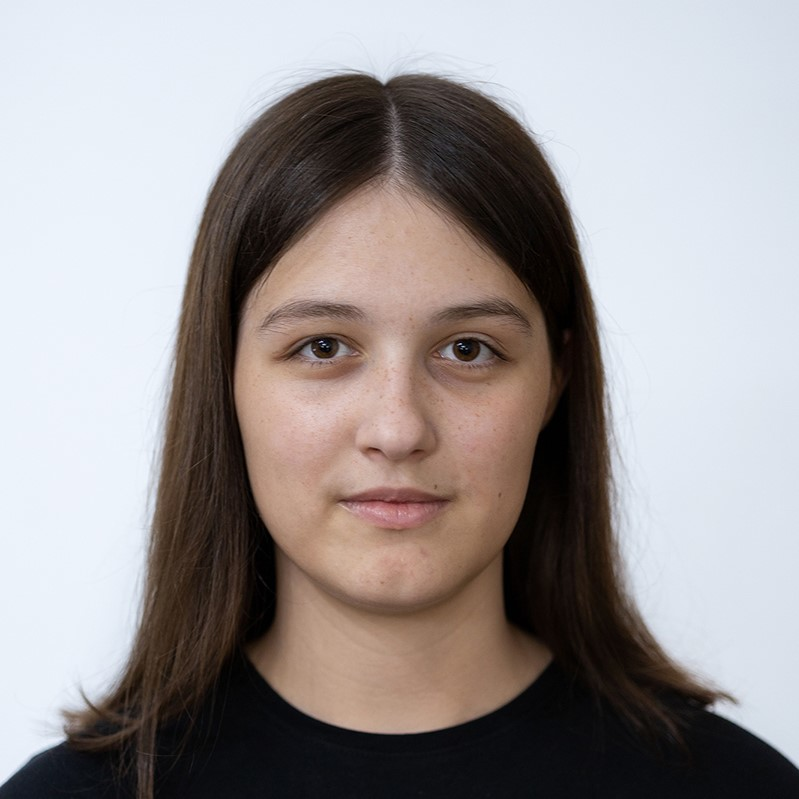
\includegraphics[width=3.5cm]{res/cover/A104437.png} &
            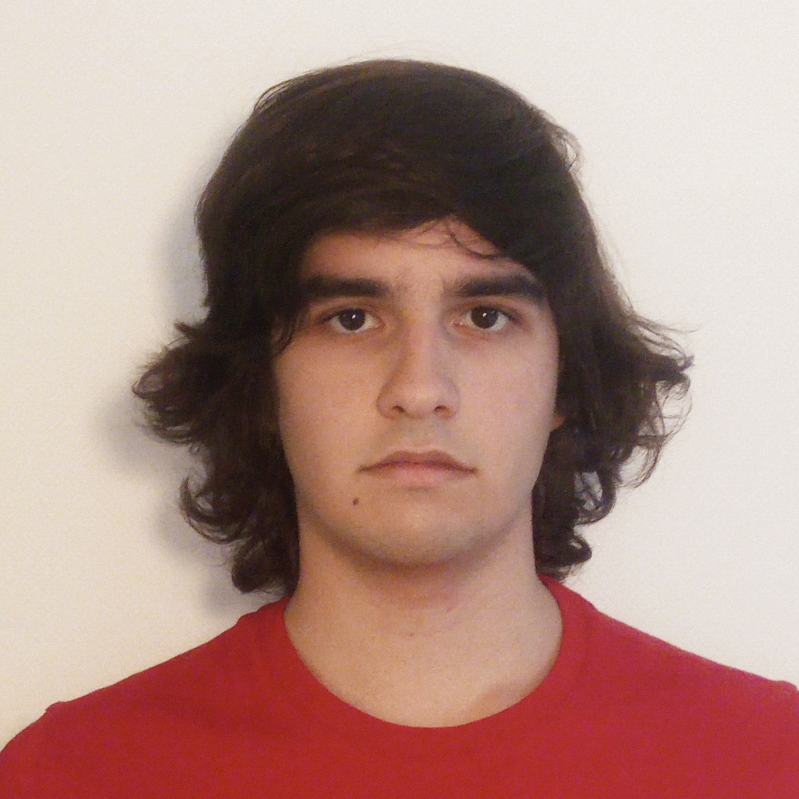
\includegraphics[width=3.5cm]{res/cover/A104348.png} &
            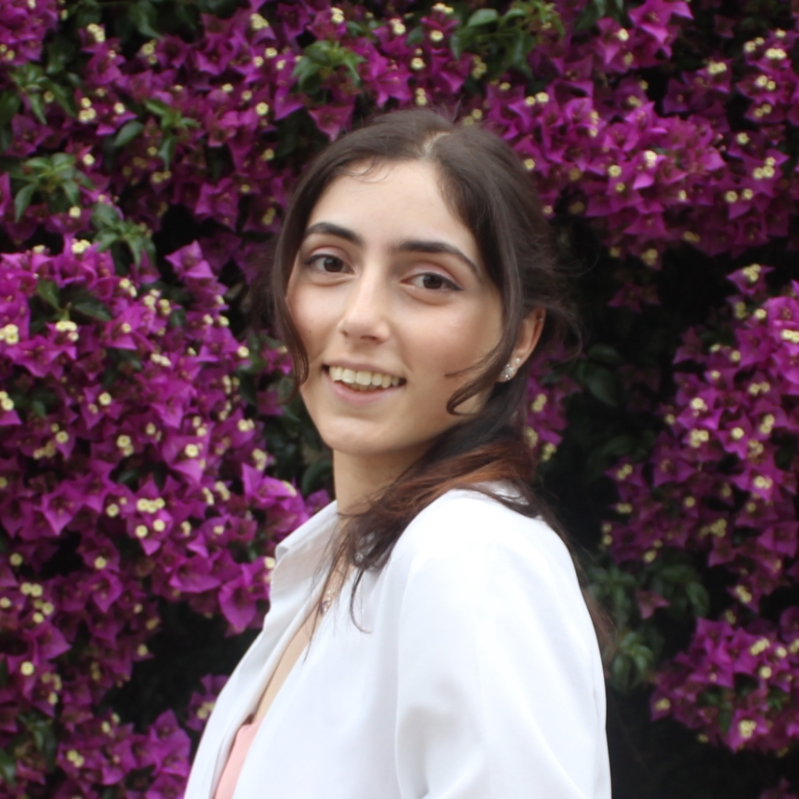
\includegraphics[width=3.5cm]{res/cover/A90817.png} &
            
\includegraphics[width=3.5cm]{res/cover/A104179.png} \\

            Ana Oliveira & Humberto Gomes & Mariana Cristino & Sara Lopes \\
            A104437      & A104348        & A90817           & A104179
        \end{tabular}
    \end{center}
\end{adjustwidth}

\pagebreak

\begin{abstract}
    \textbf{\color{red} TODO - resumo}
\end{abstract}

\section{Transformações}

\textbf{\color{red} TODO - transformações}

\section{Modelo estático do sistema solar}

\textbf{\color{red} TODO - sistema solar}

\section{Extras}

\subsection{Garrafa de Klein}

A garrafa de Klein é uma superfície não orientável, ou seja, não possui um lado interno e externo
distinguíveis. Esta não possui fronteira e trata-se de uma variedade bidimensional onde não se pode
definir um vetor normal em todos os pontos.

\subsubsection{Geração dos vértices}

Para a geração da garrafa de Klein, a superfície foi discretizada com a utilização de coordenadas
paramétricas, com o auxílio de duas variáveis ($\theta$ e $\phi$).

A parametrização de um vértice sobre a garrafa de klein de raio $r$ pode ser definida pelas
seguintes equações \cite{bottleKlein}:

$$
x = r \left( \frac{-2}{15} \right) \cos(\theta) \left(3 \cos(\phi) - 30 \sin(\theta) +
90 \cos^4(\theta) \sin(\theta) - 60 \cos^6(\theta) \sin(\theta) +
5 \cos(\theta) \cos(\phi) \sin(\theta) \right)
$$

$$
y = r \left( \frac{-1}{15} \right) \sin(\theta) \left( 3 \cos(\phi) - 3 \cos^2(\theta) \cos(\phi)
- 48 \cos^4(\theta) \cos(\phi) + 48 \cos^6(\theta) \cos(\phi) - 60 \sin(\theta) \right.
$$
$$
\quad \left. + 5 \cos(\theta) \cos(\phi) \sin(\theta) - 5 \cos^3(\theta) \cos(\phi) \sin(\theta)
- 80 \cos^5(\theta) \cos(\phi) \sin(\theta) + 80 \cos^7(\theta) \cos(\phi) \sin(\theta) \right)
$$

$$
z = r \left( \frac{2}{15} \right) (3 + 5 \cos(\theta) \sin(\theta)) \sin(\phi)
$$

A variável $\theta$ varia entre $0$ e $\pi$ e $\phi$ varia entre $0$ e $2\pi$. Além disso, o
intervalo de valores de $\theta$ e $\phi$ varia de acordo com o número de slices e stacks.

\subsubsection{Construção das faces}

Após a geração dos vértices, constroem-se as faces da garrafa de Klein. Cada quadrilátero entre duas
\emph{stacks} sucessivas é dividido em duas faces triangulares:

$$
T_1 = (P_1, P_2, P_3)
\hspace{1cm}
T_2 = (P_1, P_3, P_4)
$$

\begin{figure}[H]
    \centering
    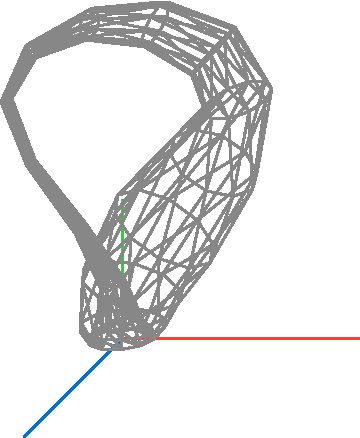
\includegraphics[width=0.3\textwidth]{res/phase2/figures/kleinBottle.pdf}
    \caption{Garrafa de Klein}
\end{figure}

\section{Resultados obtidos}

\textbf{\color{red} TODO - resultados}

\section{Conclusão e Trabalho Futuro}

\textbf{\color{red} TODO - conclusão}

\begingroup
\section{Bibliografia}
\renewcommand{\section}[2]{}

\begin{thebibliography}{9}
    \bibitem{bottleKlein}
        "Klein bottle"{} Wikipedia: Mar. 21, 2025. [Online.] Available:
        \url{https://en.wikipedia.org/wiki/Klein_bottle}
\end{thebibliography}
\endgroup

\end{document}
